\iffalse
\documentclass[12pt]{article}
\usepackage{graphicx}
%\documentclass[journal,12pt,twocolumn]{IEEEtran}
\usepackage[none]{hyphenat}
\usepackage{graphicx}
\usepackage{listings}
\usepackage[english]{babel}
\usepackage{graphicx}
\usepackage{caption} 
\usepackage{hyperref}
\usepackage{booktabs}
\def\inputGnumericTable{}
\usepackage{color}                                            %%
    \usepackage{array}                                            %%
    \usepackage{longtable}                                        %%
    \usepackage{calc}                                             %%
    \usepackage{multirow}                                         %%
    \usepackage{hhline}                                           %%
    \usepackage{ifthen}
\usepackage{array}
\usepackage{amsmath}   % for having text in math mode
\usepackage{listings}
\lstset{
language=tex,
frame=single, 
breaklines=true
}
  
%Following 2 lines were added to remove the blank page at the beginning
\usepackage{atbegshi}% http://ctan.org/pkg/atbegshi
\AtBeginDocument{\AtBeginShipoutNext{\AtBeginShipoutDiscard}}
%
%New macro definitions
\newcommand{\mydet}[1]{\ensuremath{\begin{vmatrix}#1\end{vmatrix}}}
\providecommand{\brak}[1]{\ensuremath{\left(#1\right)}}
\providecommand{\norm}[1]{\left\lVert#1\right\rVert}
\newcommand{\solution}{\noindent \textbf{Solution: }}
\newcommand{\myvec}[1]{\ensuremath{\begin{pmatrix}#1\end{pmatrix}}}
\let\vec\mathbf
\begin{document}
\begin{center}
\title{\textbf{Circles}}
\date{\vspace{-5ex}} %Not to print date automatically
\maketitle
\end{center}
\setcounter{page}{1}
\section{11$^{th}$ Maths - Chapter 11}
\textbf{This is Problem-6 from Exercise 11.1 }

Q2. Find the centre and radius of the given circle $(\vec{x} + 5)^2 + (\vec{y} – 3)^2 = 36.$

\solution
\\
Given circle equation is
\begin{align}
	(\vec{x} + 5)^2 + (\vec{y} – 3)^2 = 36 \label{1}
\end{align}
The general equation of  the circle is 
\begin{align}
	\norm{\vec{x}}^{2} + 2\vec{u}^{\top}\vec{x} + f = 0
\end{align}
Where,
\begin{align}
	\vec{u} &= -\vec{c} \text{ and } f = \norm{\vec{u}}^{2} - r^{2}\label{3}
\end{align}
by expanding \eqref{1}
\begin{align}
	\vec{x}^2+10\vec{x}+25+\vec{y}^2-6\vec{y}+9-36&=0\\
	\norm{\vec{x}}^2+2\myvec{5 & -3}\vec{x}-2&=0\label{6}
\end{align}	
by comparing \eqref{3} to \eqref{6} we get
\fi
The circle parameters are
\begin{align}
 \vec{u}=\myvec{5\\ -3},\,
 f&=-2\\
\implies \vec{c}=\myvec{-5 \\ 3},\,
	r=\sqrt{\norm{\vec{u}}^2-f}
&= 6
\end{align}
See Fig. 
\ref{fig:chapters/11/11/1/6/Fig1}.
\begin{figure}[!h]
	\begin{center} 
	   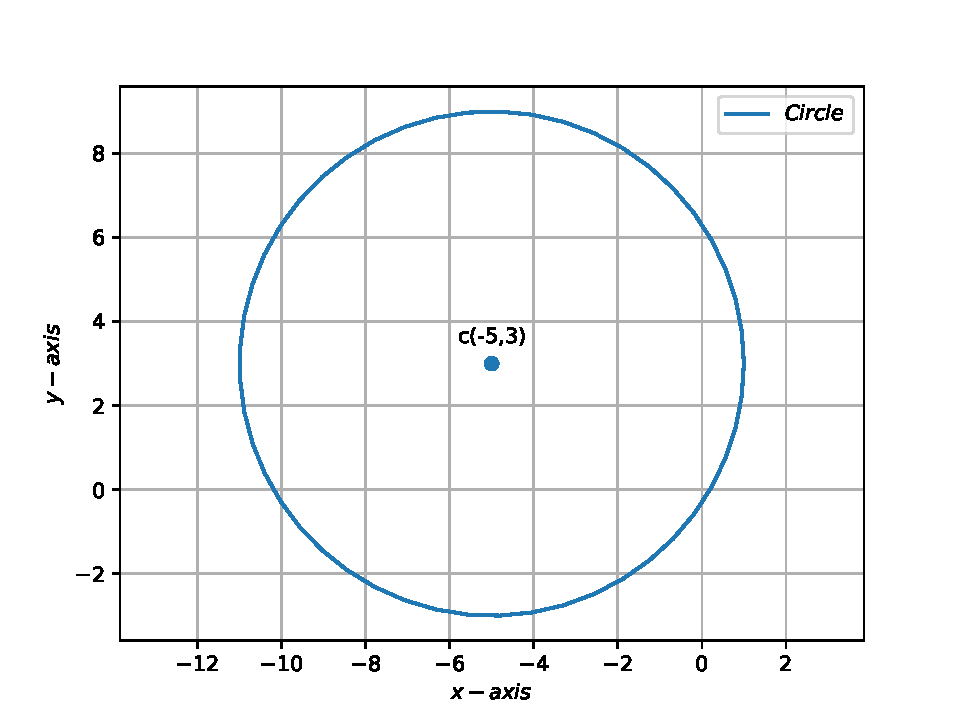
\includegraphics[width=\columnwidth]{chapters/11/11/1/6/figs/fig.pdf}
	\end{center}
\caption{}
\label{fig:chapters/11/11/1/6/Fig1}
\end{figure}

